\chapter{Spazi di n-uple e matrici}

	\section{n-uple dei numeri reali}
		\begin{comment}
		vettori numerici con n componenti
		\end{comment}
		
		I prodotti cartesiani $ \mathbb{R} \times \mathbb{R} = \mathbb{R}^2 $ e $ \mathbb{R} \times \mathbb{R} \times \mathbb{R} = \mathbb{R}^3 $, costituiti dalle coppie e terne ordinate di numeri reali, vengono utilizzati in geometria analitica per descrivere i punti del piano e dello spazio.
		
		Ora generalizziamo il concetto, introducendo gli spazi di n-uple.
		
		\subsection{Definizione} 
			L'insieme
			$$ \mathbb{R}^n = \{ a = (a_{1}, ..., a_{n}) | a_{1}, ..., a_{n} \in \mathbb{R} \} $$
			è detto spazio delle \textit{n}-uple di numeri reali, anche dette \textit{vettori numerici} a \textit{n} componenti.
		
		\subsection{Operazioni}
			Dato $ (\mathbb{R}^n, +) $ come gruppo cumulativo, esso rispetta le seguenti proprietà:
			\begin{enumerate}
				\item $ ( a + b ) + c = a + ( b + c ) $ ;
				\item \textit{n}-upla nulla $ \textbf{O} = (0, ..., 0) $ ;
				\item \underline{\textit{n}-upla opposta} di $ a \in \mathbb{R}^n $ : $ - a = ( -a_{1}, ..., -a_{n} ) $ ;
				\item $ a + b = b + a $
			\end{enumerate}
			\paragraph{osservazione} $ 1 \times a = a \quad a \in \mathbb{R}^n \wedge (-1) \times a = -a $
		
		\subsection{Proprietà con gli scalari}
			\begin{enumerate}
				\item $ k \times ( a + b ) = k \cdot a + k \cdot b  \qquad \forall k \in \mathbb{R}, \quad \forall a, b \in \mathbb{R}^n$
				\item $ ( k_{1} + k_{2} ) \times a = k_{1} \cdot a + k_{2} \cdot a  \qquad \forall k_{1}, k_{2} \in \mathbb{R}, \quad \forall a \in \mathbb{R}^n$
				\item $ ( k_{1} \cdot k_{2} ) \times a = k_{1} \times ( k_{2} \cdot a ) = k_{2} \times ( k_{1} \cdot a )  \qquad \forall k_{1}, k_{2} \in \mathbb{R}, \quad \forall a \in \mathbb{R}^n$
			\end{enumerate}
	
	\section{Matrici}
		\begin{comment}
		reali
		\end{comment}
		
		\subsection{matrici $ m \times n $ ( o di tipo (m, n) )}
			Siano $ m, n \in \mathbb{N} $, una matrice di tipo reale (m, n) è una tabella rettangolare di \textit{mn} numeri reali costituita da \textit{m} righe e \textit{n} colonne.
			
			$$
			A = 
			\begin{bmatrix}
				a_{1,1} & a_{1,2} & ... & a_{1,n} \\
				a_{2,1} & a_{2,2} & ... & a_{2,n} \\
				... & ... & ... & ... \\
				a_{m,1} & a_{m,2} & ... & a_{m,n}
			\end{bmatrix}
			$$
			
			Usiamo la notazione $ A = [ a_{ij}] $ per indicare una matrice \textit{A}, di elementi $ a_{ij} $, dove il primo indice indica la riga ed il secondo indica la colonna.
			
			\paragraph{insieme delle matrici \textit{(m, n)}:} rappresentato con il simbolo $ M_{m,n} (\mathbb{R}) $.
			
			\paragraph{classificazione in base alla lunghezza di \textit{m} e \textit{n}:}
			Una matrice di tipo (1, \textit{n}) può essere identificato con la \textit{n}-upla
			$$ (a_{11}, a_{12}, ..., a_{1n}) \in \mathbb{R}^n $$
			e viene indicata come \textit{vettore riga}, mentre una matrice di tipo (\textit{m}, 1) viene chiamata \textit{vettore colonna} e può essere identificata con la \textit{m}-upla
			$$ (a_{11}, a_{21}, ..., a_{m1}) \in \mathbb{R}^m $$
			Se $ m = n $ la matrice viene detta \textit{matrice quadrata}. Useremo il simbolo $ M_{n} (\mathbb{R}) $ per indicare l'insieme delle radici quadrate $ n \times n $. Infine una matrice $ 1 \times 1 $ sarà sempre indicata con lo scalare $ a_{11} $.
			
		\subsection{Operazioni sulle matrici}
			\begin{enumerate}
				\item \textbf{somma:}
				$$ A, B \quad (m, n), \qquad A + B = [a_{ij}] + [b_{ij}] = [a_{ij} + b_{ij}] $$
				\item \textbf{moltiplicazione per scalare:}
				$$ k \in \mathbb{R}, A (m, n) \quad k \cdot A = [k \cdot a_{ij}] $$
			\end{enumerate}
		
		\subsection{Osservazioni}
			Viene detta \underline{matrice nulla} $ 0 \in M_{m, n} (\mathbb{R}) $ quella matrice con elementi tutti nulli ed essa è \textbf{elemento neutro}. Inoltre viene denominata \underline{matrice opposta} di un'altra matrice, quella matrice $ -A = (-1) \cdot A = [-a_{ij}] $.
	
	\section{Prodotto di matrici}
		Siano A e B matrici \underline{conformabili}, ovvero matrici che hanno almeno una dimensione con la stessa lunghezza: per esempio una matrice A di tipo $ m \times n $ e B di tipo $ n \times r $.
		
		Il prodotto di A e B è la matrice $ C = A \cdot B $ di tipi $ m \times r $ con elementi
		$$ c_{ik} = \sum_{h=1}^n a_{ih} \cdot b_{hk} $$
		dove \textit{k} rappresenta la \textit{k}-esima colonna di B e \textit{i} rappresenta la \textit{i}-esima riga di A.
		
		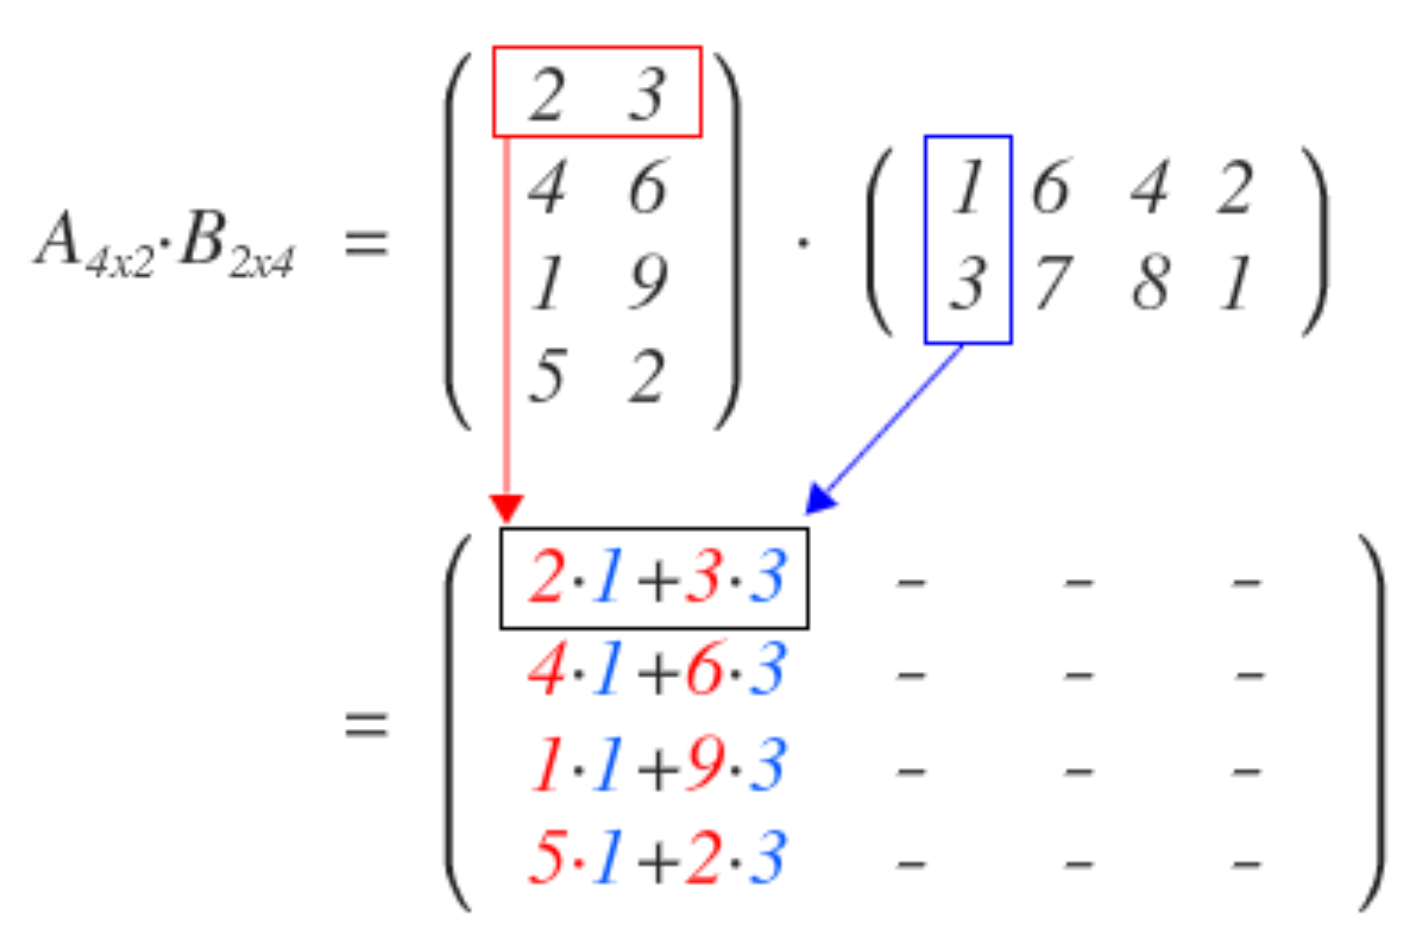
\includegraphics[width=\textwidth]{prodotto-di-matrici}
		
		\subsection{Osservazione}
			Dato un sistema composto da 3 equazioni con tre incognite, come il seguente:
			$$
			\begin{cases}
				x_1 + x_2 + x_3 = 4 \\
				2x_1 + 2x_2 + 5x_3 = 11 \\
				4x_1 + 6x_2 + 8x_3 = 24 
			\end{cases}
			$$
			
			è possibile descriverlo con due matrici: una matrice $ 3 \times 3 $, detta \textbf{matrice dei coefficienti} del sistema, descrive le incognite; mediante un vettore riga è possibile descrivere i termini noti del sistema: il sistema diviene dunque il seguente:
			$$
			A = 
			\begin{bmatrix}
				1 & 1 & 1 \\
				2 & 2 & 5 \\
				4 & 6 & 8
			\end{bmatrix}, \qquad
			b = 
			\begin{bmatrix}
				4 \\
				11 \\
				24
			\end{bmatrix}
			$$
			
			Per riottenere il sistema originale è necessario moltiplicare il sistema A con un sistema di incognite x:
			$$
			x =
			\begin{bmatrix}
				x_1 \\
				x_2 \\
				x_3
			\end{bmatrix}, \qquad
			A \cdot x =
			\begin{bmatrix}
				x_1 + x_2 + x_3 \\
				2x_1 + 2x_2 + 5x_3 \\
				4x_1 + 6x_2 + 8x_3
			\end{bmatrix}
			= b
			$$
		
		\subsection{Proprietà}
			Le proprietà del prodotto fra matrici sono le seguenti:
			\begin{enumerate}
				\item $ (AB) \cdot C = A \cdot (BC) $  associativa;
				\item $ (A + B) \cdot C = AC + BC $ distributiva;
				\item $ k \cdot (AB) = (kA) \cdot B = A \cdot (kB) \qquad \forall k \in \mathbb{R}, \forall A, B $.
			\end{enumerate}
			Com'è possibile denotare, il prodotto \textbf{non} è commutativo e dunque l'ordine delle operazioni conta (ciò non vale per tutte le coppie di matrici).
			
			\paragraph{Esempio}
			$$
			\begin{bmatrix}
				1 & 0 \\ 
				1 & 0
			\end{bmatrix}
			\begin{bmatrix}
				0 & 1 \\ 
				0& 1
			\end{bmatrix}
			=
			\begin{bmatrix}
				0 & 1 \\
				0 & 1
			\end{bmatrix}
			$$ $$ \neq $$ $$
			\begin{bmatrix}
				0 & 1 \\
				0 & 1
			\end{bmatrix}
			\begin{bmatrix}
				1 & 0 \\ 
				1 & 0
			\end{bmatrix}
			=
			\begin{bmatrix}
				1 & 0 \\ 
				1 & 0
			\end{bmatrix}
			$$
			
			\paragraph{Osservazione} Sia \textit{A} una matrice quadrata $ n \times n $ e $ k \in \mathbb{N} $ uno scalare,
			$$ A^k = \underbrace{A \cdot A \cdot ... \cdot A}_{k-volte} \text{  potenza \textit{k}-esima di \textit{A}}$$
			
			$$ A^k A^h = A^{k+h} $$
	
	\section{Tipi di matrice}
	
		\subsection{Matrice identica}
			La \textbf{matrice identica} (o \textit{matrice identità}) di ordine \textit{n} è
			$$ 
			\underbrace{I_n}_{n \times n} =
			\begin{bmatrix}
				1 & 0 & 0 & 0 \\
				0 & 1 & 0 & 0 \\
				0 & 0 & 1 & 0 \\
				0 & 0 & 0 & 1
			\end{bmatrix}_{n \times n}
			$$
			Tale matrice è simmetrica ed il suo prodotto con una matrice \textit{A} avente una dimensione uguale al lato della matrice è uguale alla matrice \textit{A}. Ciò avviene perché il prodotto fra gli elementi $ a_{ij} $ ed il corrispettivo nella matrice identità è pari ad $ a_{ij} $ stesso, gli altri prodotti sono pari all'elemento nullo.  
			$$ \implies \quad \underbrace{A}_{m \times n} \cdot I_n = A \quad \wedge \quad A \cdot I_m = A $$
		
		\subsection{Matrice invertibile}
			Sia $ A \quad n \times n $. \textit{A} è detta \textit{invertibile} se $ \exists B (n \times n) : AB = BA = I_n $.
			Se tale B esiste, si denota come $ A^{-1} $ e si chiama \textbf{matrice inversa} di \textit{A}.
		
			\paragraph{Osservazione} può valere $ AB = 0 $ con $ A \neq 0 , B \neq 0 $:
			$$
			\begin{bmatrix}
				1 & 1 \\ 
				1 & 1
			\end{bmatrix}
			\begin{bmatrix}
				1 & 1 \\ 
				-1 & -1
			\end{bmatrix}
			=
			\begin{bmatrix}
				0 & 0 \\
				0 & 0
			\end{bmatrix}
			$$
			Se \textit{A} e \textit{B} sono invertibili e sono quadrati $ n \times n \implies AB $ è invertibile:
			$$ (AB)(B^{-1}A^{-1}) = I_n $$ 
			\begin{GrayBox}
				\paragraph{Dimostrazione}
				$A (\underbrace{BB^{-1}}_{I_n}) A^{-1} = AA^{-1} = I_n $
			\end{GrayBox}
			
			$$ \implies (AB)^{-1} = B^{-1} A^{-1} $$
			$$ \implies (A_1 \cdot ... \cdot A_k)^{-1} = A_{k}^{-1} \cdot ... \cdot A_{1}^{-1} $$
			Quindi l'insieme delle \textbf{matrici $n \times n$ non invertibili} è un gruppo rispetto al prodotto matriciale (non commutativo) e viene denotato con $ GL = (n, \mathbb{R}) $ (gruppo generale lineare).
		
		\subsection{Matrice trasposta}
			Viene detta \textbf{matrice trasposta} di \textit{A} la matrice $ A^T = [a_{ji}] $ le cui righe sono le colonne di \textit{A}.
			\paragraph{Osservazione}
			\begin{itemize}
				\item $ (A + B)^T = A^T + B^T $
				\item $ (AB)^T = B^T \cdot A^T $
			\end{itemize}
		
		\subsection{Matrice simmetrica}
			Una matrice $A (n \times n) $ viene detta \textbf{simmetrica} se essa è simmetrica rispetto alla sua diagonale, ovvero se essa è uguale alla sua matrice trasposta ($ A = A^T $):
			$$
			\begin{bmatrix}
				a_{11} &
				\begin{tikzpicture}[baseline=(char.base)]
					\node(char)[draw,fill=yellow,
					shape=rounded rectangle,
					drop shadow={opacity=.5,shadow xshift=0pt},
					minimum width=1.8cm]
					{$a_{12}$};
				\end{tikzpicture} & ... & \begin{tikzpicture}[baseline=(char.base)]
					\node(char)[draw,fill=cyan,
					shape=rounded rectangle,
					drop shadow={opacity=.5,shadow xshift=0pt},
					minimum width=1.8cm]
					{$a_{1n}$};
				\end{tikzpicture}\\
				\begin{tikzpicture}[baseline=(char.base)]
					\node(char)[draw,fill=yellow,
					shape=rounded rectangle,
					drop shadow={opacity=.5,shadow xshift=0pt},
					minimum width=1.8cm]
					{$a_{21}$};
				\end{tikzpicture} & a_{12} & ... & a_{2n} \\
				... & ... & ... & a_{3n} \\
				\begin{tikzpicture}[baseline=(char.base)]
					\node(char)[draw,fill=cyan,
					shape=rounded rectangle,
					drop shadow={opacity=.5,shadow xshift=0pt},
					minimum width=1.8cm]
					{$a_{n1}$};
				\end{tikzpicture} & a_{n2} & ... & a_{nn} \\
			\end{bmatrix}
			$$
		
		\subsection{Combinazione lineare}
			Siano $ A_1, ..., A_k $ delle matrici $ m \times n $ e $ c_1, ..., c_k $ $ \in \mathbb{R} $ dei coefficienti.
			Viene detta \textbf{combinazione lineare} di $ A_1, ..., A_k $ la matrice $ m \times n $ risultante dalla somma dei prodotti delle \textit{k}-esime matrici con i \textit{k}-esimi coefficienti:
			
			$$ c_k \cdot A_k, c_k \cdot A_k, ..., c_k \cdot A_k \qquad , k \in \mathbb{N} $$
			
			\paragraph{Esempio}
			$$
			\begin{cases}
				x_1 + x_2 + x_3 = 4 \\
				2x_1 + 2x_2 + 5x_3 = 11 \\
				4x_1 + 6x_2 + 8x_3 = 24 
			\end{cases}
			\implies x_1 \begin{bmatrix}
				1 \\
				2 \\
				4
			\end{bmatrix} +  x_2 \begin{bmatrix}
				1 \\
				2 \\
				6
			\end{bmatrix} +  x_3 \begin{bmatrix}
				1 \\
				5 \\
				8
			\end{bmatrix} =  \begin{bmatrix}
				4 \\
				11 \\
				14
			\end{bmatrix} = b
			$$
		
	
	
	\section{Determinante di una matrice}
		Il determinante di una matrice è uno scalare ricavabile dalle matrici quadrate.
		
		Quando tale valore è differente da 0, il rango della matrice è massimo (ed essa è dunque invertibile), altrimenti tale rango è inferiore al massimo \textit{n}.
		
		\subsection{Definizione} Sia $A \in M_n (\mathbb{R})$. Il \textbf{determinante} di A è definito ricorsivamente:
			\begin{enumerate}
				\item se $n = 1\, , \; \det A = \det [a_{11}] = a_{11} $
				\item se $n \ge 1\, , $  
				$$ \det A = \sum_{i=1}^{n} a_{i1} a_{i1}^{\prime} \, , \qquad \text{con } a_{i1}^{\prime} = (-1)^{i + 1} \det A_{i1} $$
	
				Il determinante è dunque pari alla somma dei prodotti fra gli elementi della prima colonna ed il loro \emph{complemento algebrico} ($a_{i1}^{\prime}$). Il complemento algebrico rende tale formula ricorsiva, dato che questo ultimo è pari prodotto fra $(-1)^{i + 1}$ (che fa variare il segno a seconda della riga nella quale si trova il numero preso in esame) ed il determinante della matrice $A_{i1}$, ottenuta a seguito della rimozione della prima colonna e della \textit{i}-esima riga dalla matrice presa in esame.
			\end{enumerate}
	
		\subsection{Proprietà}
			\begin{enumerate}[(1)]
				\item Se \textit{B} è ottenuta dallo scambio di due righe di \textit{A}, il suo determinante è l'opposto di quello della matrice originale.
				$$ \det (S_{ij} A) = - \det A $$
				\item Se \textit{B} è ottenuta da \textit{A} a seguito della moltiplicazione di una riga con uno scalare \textit{c}, il suo determinante è pari al rapporto fra tale scalare ed il determinante della matrice originale.
				$$ \det (D_i (c) A) = c \cdot \det A $$
				\item Se \textit{B} è ottenuta da \textit{A} in seguito alla somma fra una riga ed il multiplo di un'altra, il suo determinante è uguale a quello della matrice originale.
				$$ \det (E_{ij}(c)A) = \det A $$
				\item se la matrice ha due righe uguali o una riga nulla, ed ha dunque un rango non massimo, il suo determinante \underline{è pari a 0}.
				\item dato $k \in \mathbb{K}$, il determinante del prodotto fra una matrice e tale scalare è pari al prodotto fra $k^n$ (dove \textit{n} è la dimensione della matrice) ed il determinante della matrice. Ciò vale grazie alla proprietà (2), dato che tale scalare viene moltiplicato per tutte le \textit{n} righe.
				$$ \det (k \cdot A) = k^n \det A $$
			\end{enumerate}
			
			Quando la matrice presa in esame è una matrice identica, le prime tre proprietà sono le seguenti:
			\begin{enumerate}[(1')]
				\item $\det (S_{ij}) = -1 $
				\item $\det (D_i (c)) = c $
				\item $\det (E_{ij} (c)) = 1 $
			\end{enumerate}
		
		\subsection{Teorema di Binet}
			Date due matrici quadrate con le stesse dimensioni, il determinante del loro prodotto matriciale è pari al prodotto fra i determinanti delle due matrici.
			$$ \det (A B) = (\det A) \cdot (\det B) \: , \qquad \forall A, B \in M_n$$
			
			\subsubsection{Corollario}
				mediante il precedente teorema è possibile affermare che il determinante di una matrice inversa è uguale all'inverso del determinante della matrice:
				$$ \det (A^{-1}) = \frac{1}{\det A} $$
			
		\subsection{Teorema}
			Il determinante di una matrice è pari al determinante della sua matrice trasposta:
			$$ \det (A^T) = \det A $$
			Questo teorema è importante perché ci permette di estendere alle colonne l'uso delle proprietà precedentemente enunciate.
				
		\subsection{Matrice a scalini} 
			Il determinante di una matrice è diverso da zero se e solo se lo è anche quello di una matrice a scalini \textit{S} ricavata dalla matrice; in tal caso il rango della matrice è massimo e dunque la matrice è invertibile.
			$$ \det A \neq 0 \iff \det S \neq 0 \iff \text{rg} A = n \iff A \text{ è invertibile}  $$
		
		\begin{GrayBox}
			\paragraph{Dimostrazione}
			è possibile ricavare una matrice a scalini \textit{S} a seguito di una serie di operazioni elementari
			$$ S = E_k \dots E_1 A $$
			dunque, per il teorema di Binet, il suo determinante è
			$$ \det S = (\det E_k) \dots (\det E_1) (\det A) $$
			Per le proprietà (1'), (2') e (3') è possibile dire che il determinante delle matrici elementari non è mai nullo e dunque, è possibile dire che affinché il determinante di \textit{S} sia pari a 0, il determinante di \textit{A} lo deve essere.
		\end{GrayBox}
	
	\subsection{Sviluppi di Laplace del determinante}
		Sia $1 \leq j \leq n$ un numero finito,
		$$ \det A = \sum_{i = 1}^{n} a_{ij} a_{ij}^{\prime} \, , \quad \text{con } a_{ij}^{\prime} = (-1)^{i + j} \det A_{ij} $$
		Sia $1 \leq i \leq n$ un numero finito,
		$$ \det A = \sum_{j = 1}^{n} a_{ij} a_{ij}^{\prime} $$
		
		\begin{GrayBox}
			\paragraph{Esempio} Sviluppiamo la seconda riga
			$$ 
			\det \begin{bmatrix}
				3 & 2 & 2 \\
				3 & 0 & 1 \\
				3 & 1 & 2
			\end{bmatrix}
			= 3 \left(- \det \begin{bmatrix}
				2 & 2 \\
				1 & 2
			\end{bmatrix} \right)
			+ 1 \left(- \det \begin{bmatrix}
				3 & 2 \\
				3 & 1
			\end{bmatrix} \right)
			= -3 \cdot (4 - 2) - 1 \cdot (3 - 6) = -3
			$$
		\end{GrayBox}

	\section{I grafi}
	
		\begin{wrapfigure}{l}{2cm}
			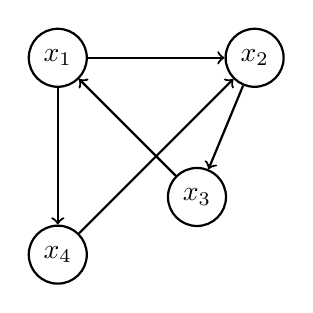
\begin{tikzpicture}[node distance={25mm}, thick, main/.style = {draw, circle}] 
				\node[main] (1) {$x_1$}; 
				\node[main] (2) [right of=1] {$x_2$}; 
				\node[main] (3) [below right of=1] {$x_3$}; 
				\node[main] (4) [below of=1] {$x_4$};  
				\draw[->] (1) -- (2);
				\draw[->] (1) -- (4);
				\draw[->] (2) -- (3);
				\draw[->] (3) -- (1);
				\draw[->] (4) -- (2);
			\end{tikzpicture}
		\end{wrapfigure}
	
		$$ V = {v_1, v_2, v_3, v_4 } \text{(insieme di vertici)} $$
		$$ E = {(1,2), (2,3), (3,1), (1,4), (4,2)} \text{(insieme dei cammini)} $$
		
		La matrice che rappresenta un grafo è denominata \textbf{matrice delle adiacenze}, tale matrice è quadrata, nelle sue righe viene indicato il peso del cammino che parte dal nodo della \textit{i}-esima riga e arriva al nodo della \textit{j}-esima colonna.
		
		$$
		A =
		\begin{bmatrix}
			0 & 1 & 0 & 1 \\
			0 & 0 & 1 & 0 \\
			1 & 0 & 0 & 0 \\
			0 & 1 & 0 & 0
		\end{bmatrix}
		$$
		
		La matrice delle adiacenze è \textit{simmetrica} se il grafo \textbf{non} è orientato.
		
		\subsection{Teorema}
			L'elemento \textit{(i, j)} della potenza $ A^{s} $ è uguale al numero di cammini di lunghezza \textit{s} dal vertice $V_i$ al vertice $V_j$.
			
			\begin{GrayBox}
				\paragraph{Dimostrazione}
				Dato $ s = 2 $ ed un nodo $V_k$, il numero di cammini di lunghezza 2 e passanti per $V_k$ è $a_{ik} \cdot a_{kj}$.
				Dato che il nodo $V_k$ può essere qualsiasi nodo ed i due nodi \textit{i} e \textit{j} sono costanti, esplicitiamo la precedente equazione rispetto ad essi:
				$$ \sum_{k=1}^n a_{ik} \cdot a_{kj} = (A^2)_{ij} $$
			\end{GrayBox}
	
	\section{Prodotto scalare in $\mathbb{R}^n$}
		Dati $x,y \in \mathbb{R}^n $, il \textbf{prodotto scalare} fra di essi è
		$$ 
		x \cdot y = \sum_{i=1}^n x_iy_i =
		\underbrace{
			\begin{bmatrix}
				x_1 & ... & x_n
			\end{bmatrix}
			\begin{bmatrix}
				y_1 \\
				... \\
				y_n
			\end{bmatrix}
		}_{\text{matrice } 1 \times 1 \implies \text{scalare}}
		=
		\begin{bmatrix}
			x_1 & ... & x_n
		\end{bmatrix}
		\begin{bmatrix}
			y_1 & ... & y_n
		\end{bmatrix}^T
		$$
		
		\subsection{Proprietà}
			\begin{enumerate}
				\item \underline{bilineare}: $ (\alpha x + \beta y) \cdot z = \alpha (x \cdot z) + \beta (y \cdot z)  $ con $ \alpha, \beta \in \mathbb{R} $ e $ x, y, z \in \mathbb{R}^n $
				\item $ x \cdot y = y \cdot x $
				\item \underline{definito positivo}: $ x \cdot x = \sum_{i=1}^n x^2_i \geq 0 $ e $ x \cdot x = 0 \iff x = 0 $
			\end{enumerate}
		
		\subsection{Norma (o lunghezza)}
			Date le precedenti proprietà è possibile definire la \textit{lunghezza} (o \textit{norma}) di $ x \in \mathbb{R}^n $ come
			$$ \Vert x \Vert = \sqrt{x \cdot x} \geq 0 $$
			Mediante la norma è dunque possibile definire pure la \textit{distanza} fra due \textit{n}-uple $x, y \in \mathbb{R}^n$ nella seguente maniera
			$$ d(x, y) = \Vert x - y \Vert \geq 0 $$
			\begin{GrayBox}
				Ciò funziona perché, facendo uso della definizione della norma e del prodotto scalare in $\mathbb{R}^2$, possiamo rappresentare tale formula come
				$$ \Vert x - y \Vert = \sqrt{(x - y)\cdot(x - y)} = \sqrt{\sum_{i=1}^{n}(x_i - y_i)^2} $$
				che è uguale alla formula che viene utilizzata per calcolare la distanza tra due punti nel piano mediante il teorema di Pitagora.
			\end{GrayBox}
		
			\paragraph{Proprietà}
			\begin{enumerate}
				\item La norma del prodotto fra una \textit{n}-upla ed uno scalare è pari al prodotto fra il modulo dello scalare e la norma della \textit{n}-upla, ovvero \newline
				$\Vert \alpha x \Vert = \vert \alpha \vert \, \Vert x \Vert $ \newline
				$\Vert \alpha x \Vert^2 = (\alpha x) \cdot (\alpha x) = \underbrace{\alpha^2}_{\sqrt{\alpha^2} = \vert \alpha \vert} \cdot \underbrace{(x \cdot x)}_{\sqrt{x \cdot x} = \Vert x \Vert} $ \newline
				Detto ciò possiamo normalizzare un vettore $v \neq 0, v \in \mathbb{R}^n$, ovvero possiamo modificarlo per far sì che la sua lunghezza sia pari ad uno:
				$$v' = \frac{1}{\Vert v \Vert} \cdot v$$
				$$\Vert v' \Vert = \frac{1}{\Vert v \Vert} \cdot \Vert v \Vert = 1$$
				$v'$ prende il nome di \textbf{versore} di \textit{v} ed è pari al rapporto fra il vettore originale e la sua lunghezza.
				\item il quadrato della lunghezza della somma di due vettori è pari alla somma fra il quadrato dei due vettori ed il doppio prodotto scalare.
				\begin{GrayBox}
					$$ \Vert x + y \Vert^2 = (x + y) \cdot (x + y) = x \cdot (x + y) + y \cdot (x + y) = x \cdot x + \underbrace{x \cdot y + y \cdot x}_{\text{doppio prodotto scalare}} + y \cdot y $$
					$$ \implies \Vert x \Vert^2 + 2 \; x \cdot y + \Vert y \Vert^2 $$
				\end{GrayBox}
				
				Lo stesso vale per il quadrato della norma della differenza fra due vettori, l'unica differenza sta nel fatto che il doppio prodotto è opposto rispetto a quello della somma (la norma di $-y$ è uguale alla norma di $y$ per la prima proprietà).
				$$ \Vert x - y \Vert^2 = \Vert x \Vert^2 - 2 \; x \cdot y + \Vert y \Vert^2 $$
				
				Dati i precedenti valori è possibile ricavare la differenza fra di essi, pari al quadruplo prodotto fra i vettori:
				$$ \Vert x + y \Vert^2 - \Vert x - y \Vert^2 = 4 \; x \cdot y $$
				
				Inoltre è possibile dire che, se \textit{x} e \textit{y} sono ortogonali, il loro prodotto è pari a 0, e dunque il quadrato della norma della somma dei due vettori è pari alla somma dei quadrati delle norme di essi (teorema di Pitagora).
				\begin{GrayBox}
					$$x \bot y \implies x \cdot y = 0 \implies \Vert x + y \Vert^2 = \Vert x \Vert^2 + \Vert y \Vert^2 $$
				\end{GrayBox}
			\end{enumerate}
			
			
			\subsection{Proiezione di un vettore su un altro vettore}
				Dati i vettori $ x, y \in \mathbb{R}^n, \quad y \neq 0 $ ed uno scalare $ c \in \mathbb{R} \ $
				$$ x - cy \, \bot \, y \implies (x - cy) \cdot y = 0 $$
				Sviluppando l'equazione risulta che lo scalare c è pari al rapporto fra il prodotto scalare fra i due vettori ed il prodotto fra il vettore nel quale si deve effettuare la proiezione per sè stesso (sappiamo, data la definizione della norma, che il prodotto di un vettore con sè stesso è pari al quadrato della sua lunghezza).
				$$ \implies x \cdot y - c \, ( y \cdot y)  = 0 $$
				$$ \implies c = \frac{x \cdot y}{y \cdot y}$$
				
				\begin{center}
					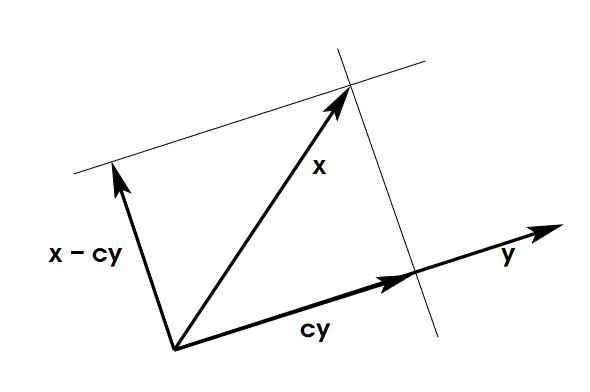
\includegraphics[width=\textwidth/2]{proiezione-vett-x-y}
				\end{center}
				
				Moltiplicando lo scalare precedentemente trovato con il vettore nel quale deve essere effettuata la proiezione, è possibile ottenere la \textbf{proiezione ortogonale} su x su y, chiamato anche \textit{vettore proiezione}.
				$$ pr_y(x) = c \cdot y = \frac{x \cdot y}{\Vert y \Vert^2} \cdot y \in \mathbb{R}^n $$
			
			\subsection{Disuguaglianza di Cauchy-Schwanz}
				Tale disuguaglianza afferma che il modulo del prodotto fra due vettore è minore (o uguale) al prodotto fra le norme dei vettori.
				$$ \vert x \cdot y \vert \leq \Vert x \Vert \cdot \Vert y \Vert \qquad \forall x, y \in \mathbb{R}^n $$
				I termini risultano uguale se e solo \textit{x} e \textit{y} sono proporzionali, ovvero 
				$$ x = \lambda \cdot y \, , \; \forall \lambda \in \mathbb{R} $$
				
				\begin{GrayBox}
					\paragraph{Dimostrazione} se $ y = 0 \implies \text{i due termini sono uguali} $ \newline
					se $ y \neq 0 \implies x = pr_y(x) + x' \, , \; \text{con } x' \bot y $ \newline
					detto ciò sappiamo che la norma di \textit{x} sarà sicuramente maggiore della norma della sua proiezione su \textit{y}, dato che essa è una degli addendi che generano x; Definito ciò possiamo dunque dire che il quadrato della norma di \textit{x} è maggiore del quadrato della norma di tale proiezione.
					$$ \Vert x \Vert^2 = \Vert pr_y(x) \Vert^2 + \Vert x' \Vert^2 \geq \Vert pr_y(x) \Vert^2 = \Vert \frac{x \cdot y}{\Vert y \Vert^2} \cdot y \Vert^2$$
					Semplificando la proiezione è possibile dire che il quadrato della norma di \textit{x} è maggiore (o uguale) al rapporto fra il quadrato del modulo del prodotto fra \textit{x} e \textit{y} e il quadrato della norma di \textit{y}.
					$$ \Vert x \Vert^2 \geq \frac{\vert x \cdot y \vert^2}{\Vert y \Vert^4} \cdot \Vert y \Vert^2 = \frac{\vert x \cdot y \vert^2}{\Vert y \Vert^2} $$
					
					Portando a sinistra il denominatore del secondo termine e mettendo tutto sotto radice, è possibile sostenere l'assunto iniziale, ovvero
					$$ \vert x \cdot y \vert \leq \Vert x \Vert \cdot \Vert y \Vert \qquad \forall x, y \in \mathbb{R}^n $$
				\end{GrayBox}
			
			\subsection{Disuguaglianza triangolare}
				Viene affermato che la lunghezza della somma di due vettori è minore (o uguale) alla somma delle loro lunghezze.
				$$ \Vert x + y \Vert = \Vert x \Vert + \Vert y \Vert \quad x, y \in \mathbb{R}^n $$
				\begin{GrayBox}
					\paragraph{Dimostrazione} La dimostrazione di questo assunto è abbastanza semplice perché sappiamo che il quadrato della lunghezza di due vettori è pari alla somma dei quadrati delle loro lunghezze ed il loro doppio prodotto, i due termini saranno uguali nei casi nei quali il doppio prodotto è nullo, ovvero quando i due vettori sono perpendicolari.
				\end{GrayBox}
				
				\subsection{Disuguaglianza triangolare per la distanza}
				La distanza fra due vettori \textit{x} e \textit{y} è sempre minore (o uguale) alla distanza fra di essi passando per un vettore \textit{z}:
				$$ d(x, y) \leq d(x, y) + d(z, y) \qquad \forall x, y, z \in \mathbb{R}^n $$
			
				\begin{GrayBox}
					La distanza fra \textit{x} e \textit{y} può essere vista come la somma della differenza fra \textit{x} e \textit{z} e la differenza fra \textit{z} e \textit{y}:
					$$ d(x, y) = \Vert x - y \Vert = \Vert (x - z) + (z - y) \Vert $$
					Invece, la distanza fra \textit{x} e \textit{y} calcolata passando per un vettore \textit{z} è pari alla somma fra la lunghezza del segmento \textit{xz} ed il segmento \textit{zy}:
					$$ d(x, z) + d(z, y) = \Vert x - z \Vert + \Vert z - y \Vert $$
					Facendo uso della disuguaglianza triangolare precedentemente dimostrata, è possibile affermare la seguente:
					$$ \Vert (x - z) + (z - y) \Vert \leq \Vert x - z \Vert + \Vert z - y \Vert $$
					E da ciò ne conviene l'assunto iniziale.
				\end{GrayBox}
			
			\subsection{Angolo compreso tra due vettori}
				Date le \textit{n}-uple \textit{x} e \textit{y} \underline{non nulle}, e sapendo che il rapporto fra il prodotto vettoriale $ x \cdot y $ ed il prodotto $ \Vert x \Vert \cdot \Vert y \Vert $ è compreso fra -1 e 1 \footnote{la disuguaglianza di Cauchy-Schwanz afferma che il modulo del primo è minore del secondo, dunque senza modulo il risultato di tale prodotto è compreso fra -1 e 1}, è possibile affermare che il risultato di tale prodotto è pari al coseno dell'angolo (convesso) compreso fra i due vettori.
				\begin{GrayBox}
					$$ -1 \leq \frac{x \cdot y}{\Vert x \Vert \cdot \Vert y \Vert} \leq 1 $$
					$$ \implies \cos \theta = \frac{x \cdot y}{\Vert x \Vert \cdot \Vert y \Vert} \: , \quad \theta \in [0, \pi] $$
				\end{GrayBox}